% Q1.1: one cable to scale (radii in mm). Each leader line ends in a dot inside its layer.
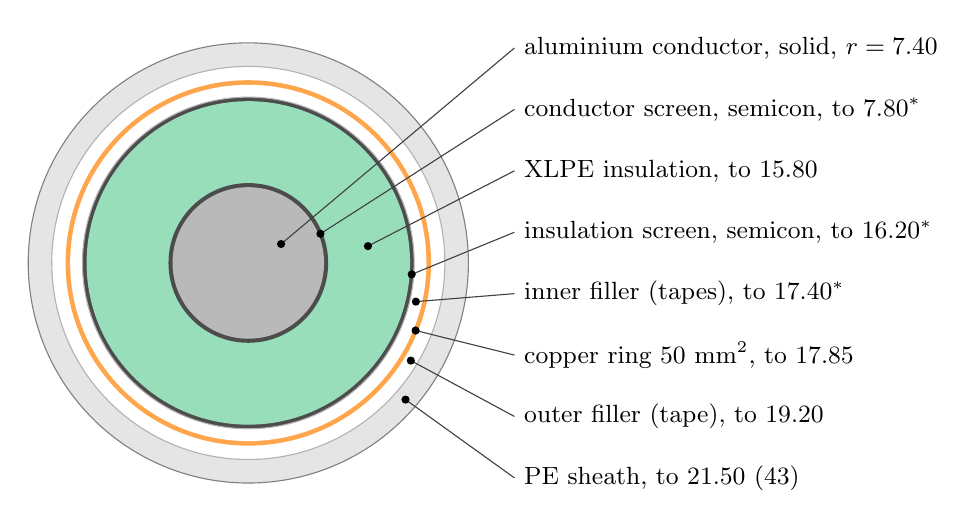
\begin{tikzpicture}[scale=0.13]
\fill[gray!20] (0,0) circle (21.5); \fill[white] (0,0) circle (19.2);
\fill[orange!70] (0,0) circle (17.85); \fill[white] (0,0) circle (17.4);
\fill[black!70] (0,0) circle (16.2); \fill[green!35!teal!40] (0,0) circle (15.8);
\fill[black!70] (0,0) circle (7.8); \fill[gray!55] (0,0) circle (7.4);
\draw[gray] (0,0) circle (21.5); \draw[gray!60] (0,0) circle (19.2); \draw[gray!60] (0,0) circle (16.2);
\foreach \r/\a/\t/\y in {3.7/30/{aluminium conductor, solid, $r=7.40$}/21,
   7.6/22/{conductor screen, semicon, to 7.80$^*$}/15, 11.8/8/{XLPE insulation, to 15.80}/9,
   16.0/-4/{insulation screen, semicon, to 16.20$^*$}/3, 16.8/-13/{inner filler (tapes), to 17.40$^*$}/-3,
   17.625/-22/{copper ring 50 mm$^2$, to 17.85}/-9, 18.52/-31/{outer filler (tape), to 19.20}/-15,
   20.35/-41/{PE sheath, to 21.50 ($\varnothing$43)}/-21}
  {\draw[thin,black!75] (26,\y) node[right,font=\small,black]{\t} -- ({\r*cos(\a)},{\r*sin(\a)});
   \fill[black] ({\r*cos(\a)},{\r*sin(\a)}) circle (0.4);}
\end{tikzpicture}
